\documentclass{beamer}

\usepackage[czech]{babel}
\usepackage[utf8]{inputenc}
\usepackage[T1]{fontenc}
\usepackage{lmodern}
\usepackage{datetime}
\usepackage{tikz}
\usepackage{amssymb}
\usepackage{bbding}
\usepackage{tabularx}
\usepackage{wrapfig}

\usetikzlibrary{shadows}
% Themes: http://www.hartwork.org/beamer-theme-matrix/
\mode<presentation>{\usetheme{Madrid}}
\usecolortheme{default}
\beamertemplatenavigationsymbolsempty 
\setbeamertemplate{title page}[default][colsep=0bp,rounded=true]
\setbeamertemplate{itemize items}{$\star$}
\setbeamercolor*{item}{fg=black}
\setbeamertemplate{enumerate item}[default]
\newcommand{\Has}{\textcolor{green}{\CheckmarkBold}}
\newcommand{\NoHas}{\textcolor{red}{\XSolidBrush}}
\newcommand{\It}{\textit}  % kurzíva
\newcommand{\B}{\textbf} %tučné písmo
\newcommand{\U}{\underline}  % podtržené písmo
\newcommand{\sectsel}[1]{\U{\B{#1}}}

\newenvironment<>{positiveblock}[1]{%
  \begin{actionenv}#2%
      \def\insertblocktitle{#1}%
      \par%
      \mode<presentation>{%
        \setbeamercolor{block title}{fg=white,bg=green!20!black}
       \setbeamercolor{block body}{fg=black,bg=green!40}
       \setbeamercolor{itemize item}{fg=green!20!black}
       \setbeamertemplate{itemize item}[triangle]
     }%
      \usebeamertemplate{block begin}}
    {\par\usebeamertemplate{block end}\end{actionenv}}
    
\newenvironment<>{negativeblock}[1]{%
  \begin{actionenv}#2%
      \def\insertblocktitle{#1}%
      \par%
      \mode<presentation>{%
        \setbeamercolor{block title}{fg=white,bg=red!20!black}
       \setbeamercolor{block body}{fg=black,bg=red!20}
       \setbeamercolor{itemize item}{fg=red!20!black}
       \setbeamertemplate{itemize item}[triangle]
     }%
      \usebeamertemplate{block begin}}
    {\par\usebeamertemplate{block end}\end{actionenv}}


\author{Vojtěch Boček}
%\institute[vbocek@gmail.com]{SPŠ a VOŠ technická, Sokolská 1, Brno \\[0.5cm] \includegraphics[width=2cm]{logo-skoly}}
\institute[vbocek@gmail.com]{SPŠ a VOŠ technická Brno, Sokolská 1}
\title{MultiROM}
\subtitle{Nástroj pro instalaci více operačních systémů\\na jedno mobilní zařízení}
\date[]{}

%\newdate{date}{13}{03}{2013}
%\date{\displaydate{date}}

\setbeamerfont{sections}{size=\fontsize{8}{9}\selectfont}

\begin{document}


\frame{\titlepage}

\begin{frame}
    \frametitle{MultiROM}
    \begin{columns}
    \column{.48\textwidth}
    \vspace{-10mm}
    \begin{itemize}
        \item Instalace libovolného množství vedlejších systémů -- \It{multiboot}
        \item Podpora mnoha operačních systémů
        \item Snadné používání
    \end{itemize}
    \column{.48\textwidth}
    \vspace{-5mm}
    \begin{figure}[H]
    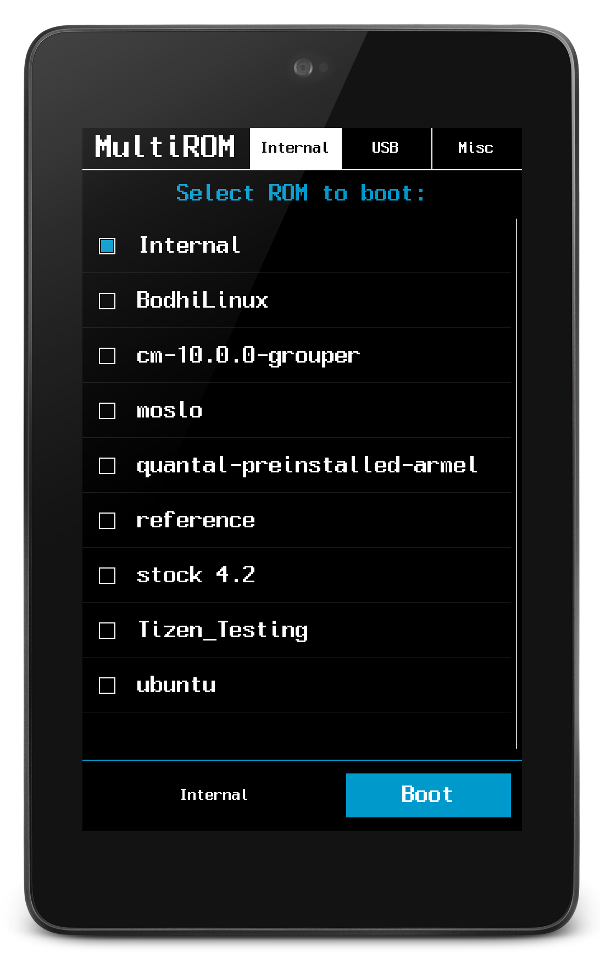
\includegraphics[width=145px]{../img/boot_manager_promo.png}
    \end{figure}
%     \begin{figure}[H]
%     \begin{tikzpicture}
%         \node[drop shadow={shadow xshift=.8ex,shadow yshift=-.8ex},fill=white,draw] at (0,0) { 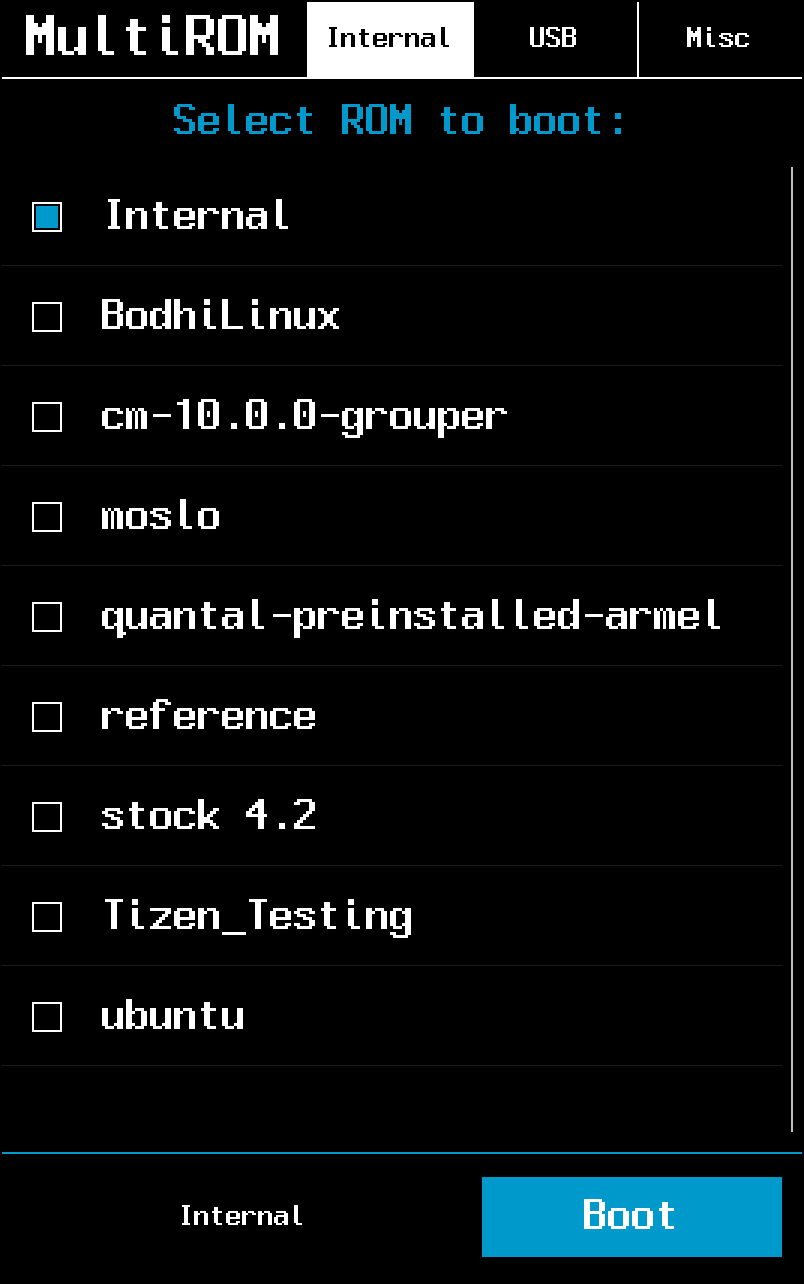
\includegraphics[width=120px]{../img/boot_manager.png}};
%     \end{tikzpicture}
%     \end{figure}
    \end{columns}
\end{frame}


\begin{frame}
    \frametitle{Aktuální stav}
    \begin{itemize}
        \item Oficiálně podporována 4 zařízení (tablety Nexus 7 2012 \& 2013 a telefony Nexus 4 a Nexus 5)
        \item Více než desítka dalších zařízení podporována komunitou
        \item Přes 15 000 aktivních instalací
        \item Úspěšný crowdfunding projekt
    \end{itemize}
    \begin{figure}[H]
    \begin{tikzpicture}
         \node[fill=white,draw] at (0,0) { 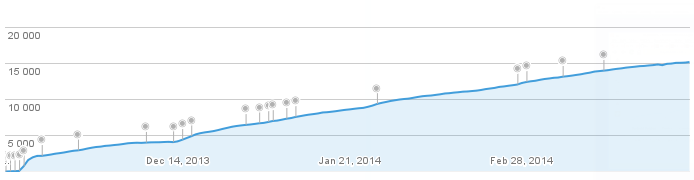
\includegraphics[width=0.95\textwidth]{../img/graph_active.png}};
    \end{tikzpicture}
    \end{figure}
\end{frame}

\begin{frame}
    \frametitle{Části projektu}
    \begin{enumerate}
        \item Boot manager
        \item Upravená recovery
        \item Kexec-hardboot patch
        \item Aplikace pro Android
    \end{enumerate}
\end{frame}

\begin{frame}
    \vspace{-2.5ex}
    \begin{beamercolorbox}[wd=\paperwidth,ht=2.5ex,dp=1.125ex,center=true]{palette quaternary}%
    \usebeamerfont{sections}
    \sectsel{1. Boot manager} | 2. Upravená recovery | 3. Kexec-hardboot patch | 4. Aplikace pro Android
    \end{beamercolorbox}
    \vspace{-1.5ex}

    \frametitle{Boot Manager}
    \begin{columns}
    \column{.48\textwidth}
    \begin{itemize}
        \item Zobrazuje se po spuštění zařízení
        \item Slouží pro výběr systému
        \item Obsahuje kód, který se stará o multiboot
        \item Umí automaticky spustit nastavený systém
    \end{itemize}
    \vspace{10mm}

    \column{.48\textwidth}
    \begin{figure}[H]
    \begin{tikzpicture}
        \node[drop shadow={shadow xshift=.8ex,shadow yshift=-.8ex},fill=white,draw] at (0,0) { 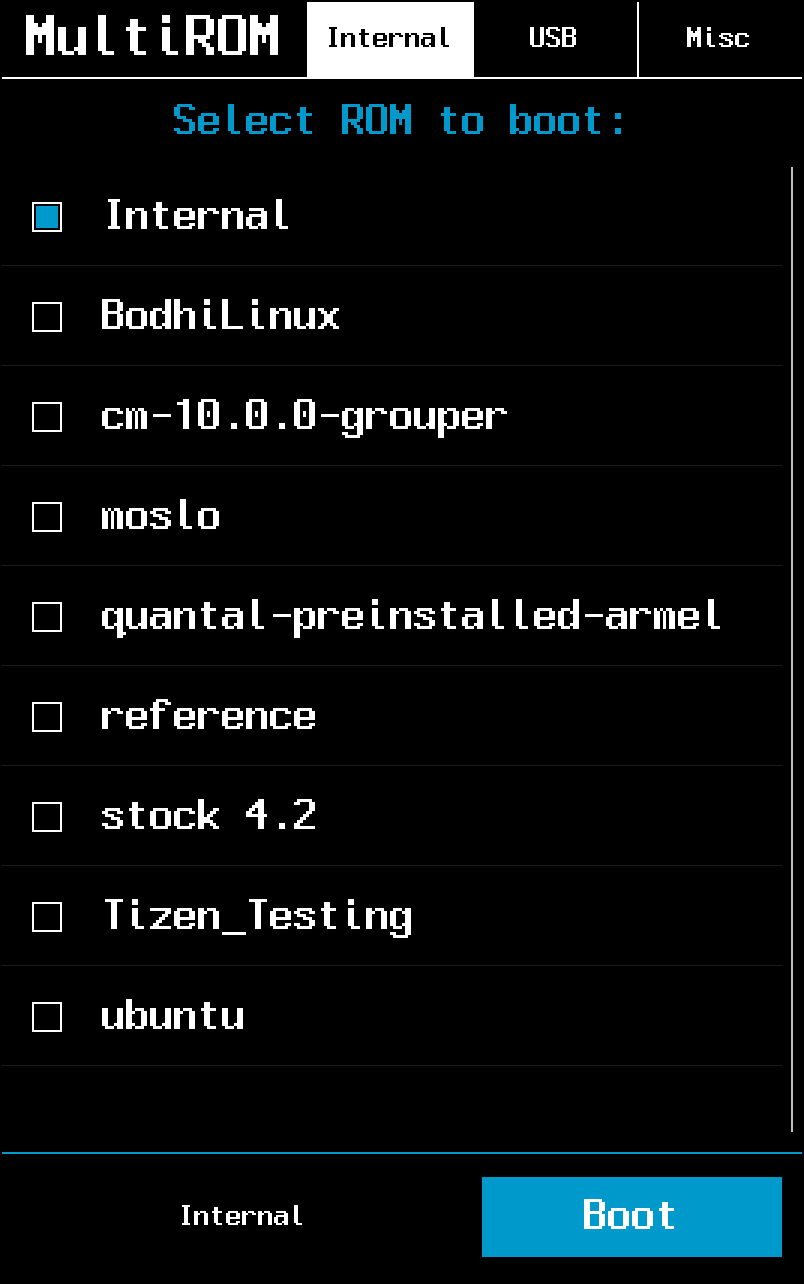
\includegraphics[width=120px]{../img/boot_manager.png}};
    \end{tikzpicture}
    \end{figure}
    \end{columns}
\end{frame}

\begin{frame}
    \vspace{-2.0ex}
    \begin{beamercolorbox}[wd=\paperwidth,ht=2.5ex,dp=1.125ex,center=true]{palette quaternary}%
    \usebeamerfont{sections}
    1. Boot manager | \sectsel{2. Upravená recovery} | 3. Kexec-hardboot patch | 4. Aplikace pro Android
    \end{beamercolorbox}
    \vspace{-1.5ex}
    
    \frametitle{Upravená recovery}
    \begin{columns}
    \column{.48\textwidth}
    \begin{itemize}
        \item Původně zejména pro opravu hlavního systému
        \item Správa vedlejších systémů
        \item Nastavení MultiROM
        \item Založená na open-source projektu TWRP
    \end{itemize}
    \vspace{10mm}

    \column{.48\textwidth}
    \begin{figure}[H]
    \begin{tikzpicture}
        \node[drop shadow={shadow xshift=.8ex,shadow yshift=-.8ex},fill=white,draw] at (0,0) { 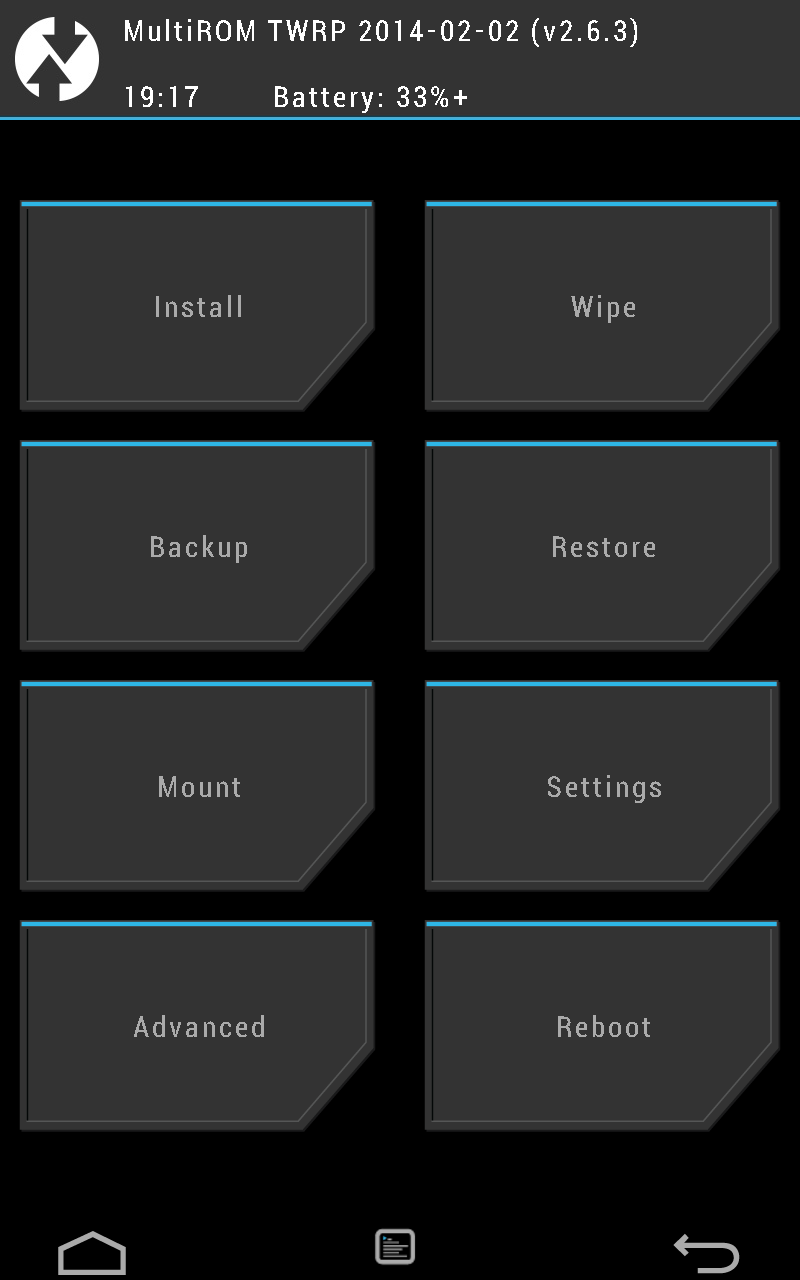
\includegraphics[width=120px]{../img/recovery.png}};
    \end{tikzpicture}
    \end{figure}
    \end{columns}
\end{frame}

\begin{frame}
    \vspace{-12.4ex}
    \begin{beamercolorbox}[wd=\paperwidth,ht=2.5ex,dp=1.125ex,center=true]{palette quaternary}%
    \usebeamerfont{sections}
    1. Boot manager | 2. Upravená recovery | \sectsel{3. Kexec-hardboot patch} | 4. Aplikace pro Android
    \end{beamercolorbox}
    \vspace{10.0ex}

    \frametitle{Kexec-hardboot patch}
    \begin{itemize}
        \item Úprava Linuxového jádra
        \item Spouštění jiného jádra s pomocí toho již běžícího
        \item Nepřepíše jádro uložené v boot sektoru
        \item Technicky umožňuje multiboot na zařízeních s tak limitovaným přístupem, jako jsou tablety a telefon s OS Android
    \end{itemize}
\end{frame}

\begin{frame}
    \vspace{-2.0ex}
    \begin{beamercolorbox}[wd=\paperwidth,ht=2.5ex,dp=1.125ex,center=true]{palette quaternary}%
    \usebeamerfont{sections}
    1. Boot manager | 2. Upravená recovery | 3. Kexec-hardboot patch | \sectsel{4. Aplikace pro Android}
    \end{beamercolorbox}
    \vspace{-1.5ex}
    
    \frametitle{Aplikace pro Android}
    \begin{columns}
    \column{.48\textwidth}
    \begin{itemize}
        \item Instalace a aktualizace MultiROM
        \item Přejmenovávání a mazání nainstalovaných systémů
        \item Bootování přímo do nainstalovaných systémů
    \end{itemize}
    \vspace{10mm}

    \column{.48\textwidth}
    \begin{figure}[H]
    \begin{tikzpicture}
        \node[drop shadow={shadow xshift=.8ex,shadow yshift=-.8ex},fill=white,draw] at (0,0) { 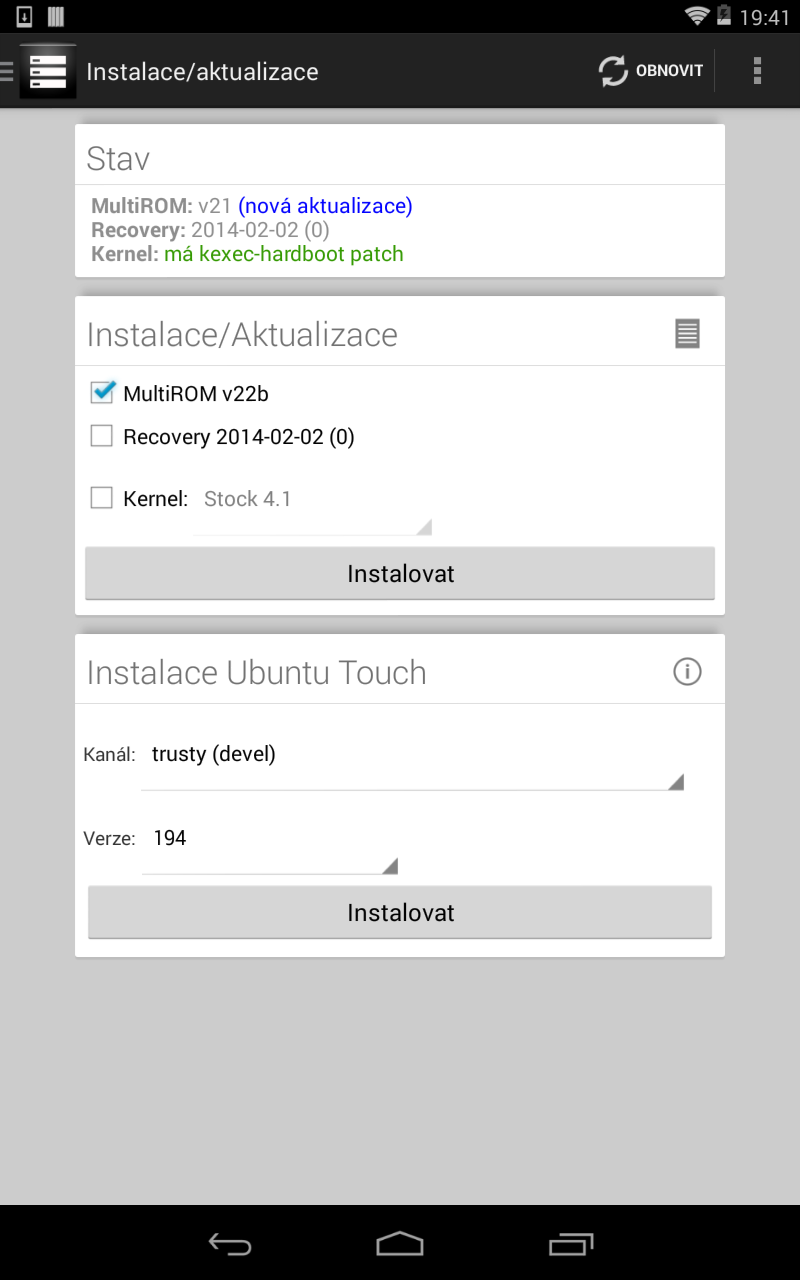
\includegraphics[width=120px]{../img/app_main.png}};
    \end{tikzpicture}
    \end{figure}
    \end{columns}
\end{frame}

% BOOT MENUp
% to stejne na N5, tam boot android
% N7 - recovery, boot android
% n5 - ukazat nabootovanou rom, reboot do ubuntu
% n7 - ukazat app a widget
% n5 - ukazat ubuntu

\begin{frame}
    \begin{center}
        {\Large *\It{Pravděpodobně} živá ukázka!* }
        \begin{figure}[H]
        
\includegraphics[width=0.4\textwidth]{../img/kocka.png}
        \end{figure}
    \end{center}
\end{frame}


\begin{frame}
    \frametitle{Porovnání s existujicími řešeními}
    \begin{positiveblock}{Výhody}
    \begin{itemize}
        \item Velmi snadné používání
        \item Libovolné množství systémů
        \item Libovolný typ systémů
        \item Instalace vedlejších systémů do vnitřní paměti nebo na USB flash disk
        \item Žádný dopad na rychlost systému
    \end{itemize}
    \end{positiveblock}

    \pause
    \begin{negativeblock}{Nevýhody}
    \begin{itemize}
        \item Nemožnost sdílení aplikací mezi systémy
    \end{itemize}
    \end{negativeblock}
\end{frame}

\begin{frame}
    \frametitle{Proč?}
    \begin{itemize}
        \item Na PC je multiboot běžná funkcionalita
        \item Vyzkoušení jiných operačních systémů
        \item Vývoj aplikací pro Android
        \item Využívání aplikací kompatibilních pouze s jedním OS
    \end{itemize}
\end{frame}

\begin{frame}
    \frametitle{Zkoušení rozdílných ROM}
    \begin{columns}
    \column{.48\textwidth}
        \begin{negativeblock}{Dříve}
            \begin{enumerate}
                \item Udělat zálohu stávajícího OS
                \item Nainstalovat nový systém
                \item Zjistit, že starý byl lepší
                \item Obnovit zálohu
                \pause
                \item Zhrozit se nad množstvím času stráveného touto operací
            \end{enumerate}
        \end{negativeblock}
    \pause
    \column{.48\textwidth}
        \begin{positiveblock}{S MultiROM}
            \vspace{3mm}
            \begin{enumerate}
                \item Nainstalovat nový systém do MultiROM
                \item[2a.] Zjistit, že starý byl lepší a smazat ho
                \pause
                \item[2b.] Hmm, ujde, zatím ho nesmažu
            \end{enumerate}
            \vspace{2mm}
        \end{positiveblock}
    \end{columns}
\end{frame}

\begin{frame}
    \frametitle{Shrnutí}
    \begin{itemize}
        \item Výrazně jednodušší používání v porovnání s ostatními podobnými modifikacemi
        \item Podpora prakticky jakéhokoliv operačního systému
%        \item Přispívání zpět do komunity, zejména TWRP a Ubuntu Touch
        \item MultiROM nebo její části využívají i další vývojáři
        \item Přes 15 000 uživatelů
        \item Úspěšný crowdfunding projekt
        \item Další vývoj:
        \begin{itemize}
            \item Podpora dalších zařízení
            \item Možnost sdílení aplikací mezi instalacemi Android ROM
        \end{itemize}
    \end{itemize}
\end{frame}


\begin{frame}
    \begin{center}
        {\huge Děkuji za pozornost}

        \vspace{20mm}
        MultiROM Manager: \\
        \url{http://bit.ly/mrom_app}
    \end{center}
\end{frame}

\end{document}